\documentclass[twoside,11pt,a4paper,leqno]{article}

% leqno put equations numbers on the left. this is not typical, but makes them easier to find because I number them in sequence with theorems.

% \usepackage[utf8]{inputenc} % should be default anyhow
% \usepackage[iso]{umlaute}
% \usepackage{theorem}
\usepackage{amsmath}
\usepackage{amsthm}
\usepackage{amssymb}
\usepackage{amsxtra}
% \usepackage{german} % darf nicht weiter oben stehen
% \usepackage[matrix,arrow]{xy}    % all
% \usepackage{makeidx}
\usepackage{fancyhdr}%  für die Seitenküpfe
% \usepackage{epsfig}
% \usepackage{curves,epic,eepic}% z.B. für groüe Kreise
% \usepackage{boxedminipage}
% \usepackage[T1]{fontenc}  % Suche in PDF, vgl. Mail von Viktor Bindewald vom 24.11.09
% \usepackage{verbatim}
% \usepackage{longtable}
\usepackage{tikz}
\usepackage{mathrsfs} % \mathscr{...}: super-cursive letters
% \usepackage{wasysym} % \smiley{}
% \usepackage{framed}
\usepackage{mdframed}
\usepackage{graphicx}
% \usepackage{enumitem}
\usepackage{hyperref}
\hypersetup{
    colorlinks=true,
    linkcolor=blue,
    % filecolor=magenta,      
    % urlcolor=cyan,
    % pdftitle={Overleaf Example},
    % pdfpagemode=FullScreen,
    }

%%%%%%%%%%%%%%%%%%%%%%%%%%%%%%%%%%%%%%%%%%%%%%
%% Page formatting
%%%%%%%%%%%%%%%%%%%%%%%%%%%%%%%%%%%%%%%%%%%%%%
\setlength{\textheight}{23cm}
\setlength{\textwidth}{16cm}
\setlength{\oddsidemargin}{0.2cm}
\setlength{\evensidemargin}{0.2cm}
% \setlength{\topmargin}{0cm}
% \setlength{\headheight}{0cm}
% \setlength{\topsep}{0pt}
% \setlength{\headsep}{1.0cm}
% \setlength{\partopsep}{0pt}
\parindent0pt
\setlength{\parskip}{0.7\baselineskip}

% Start sections on a new page
% \AddToHook{cmd/section/before}{\clearpage}

\renewcommand{\theenumi}{\alph{enumi}}
% \renewcommand*{\thefootnote}{\fnsymbol{footnote}}

%%%%%%%%%%%%%%%%%%%%%%%%%%%%%%%%%%%%%%%%%%%%%%
%% Theorem Environments
%%%%%%%%%%%%%%%%%%%%%%%%%%%%%%%%%%%%%%%%%%%%%%
\numberwithin{equation}{section}

\theoremstyle{plain}
% \newtheorem{Def}{Definition}[]
\newtheorem{definition}[equation]{Definition}
%\newtheorem{Prop}[Def]{Proposition.}
\newtheorem{theorem}[equation]{Theorem}
\newtheorem{lemma}[equation]{Lemma}
\newtheorem{corollary}[equation]{Corollary}

% \theorembodyfont{\rmfamily\mdseries\upshape}
%\newtheorem{Beispiel}[Def]{Beispiel}
\theoremstyle{definition}
\newtheorem{example}[equation]{Example}
\newtheorem{remark}[equation]{Remark}
\newtheorem{question}[equation]{Question}
\newtheorem{exercise}[equation]{Exercise}
% To end an example environment with a symbol.
% \AtBeginEnvironment{example}{%
%   \pushQED{\qed}\renewcommand{\qedsymbol}{$\triangle$}%
% }
% \AtEndEnvironment{example}{\popQED\endexample}
\newmdenv[
  leftmargin = 0pt,
  innerleftmargin = 1em,
  innertopmargin = 0pt,
  innerbottommargin = 0pt,
  innerrightmargin = 0pt,
  rightmargin = 0pt,
  linewidth = 1pt,
  topline = false,
  rightline = false,
  bottomline = false
  ]{leftbar}
\AtBeginEnvironment{example}{%
  \begin{leftbar}
}
\AtEndEnvironment{example}{\end{leftbar}}

% Force a label on a * equation environment
\newcommand{\labelthis}[1]{\addtocounter{equation}{1}\tag{\theequation}\label{#1}}

%%%%%%%%%%%%%%%%%%%%%%%%%%%%%%%%%%%%%%%%%%%%%%
%% Macros
%%%%%%%%%%%%%%%%%%%%%%%%%%%%%%%%%%%%%%%%%%%%%%

\DeclareMathOperator{\dom}{dom}
\DeclareMathOperator{\src}{src}
\DeclareMathOperator{\codom}{codom}
\DeclareMathOperator{\img}{img}
% \DeclareMathOperator{\ker}{ker}
\DeclareMathOperator{\vspan}{span}
% \DeclareMathOperator{\parto}{\rightharpoonup}
% \DeclareMathOperator{\dist}{dist}
% \DeclareMathOperator{\det}{det}
\DeclareMathOperator{\tr}{tr}
\DeclareMathOperator{\id}{id}
% \DeclareMathOperator{\Rm}{Rm}
% \DeclareMathOperator{\Ric}{Ric}
\DeclareMathOperator*{\proj}{proj}
\DeclareMathOperator{\Real}{Re}
\DeclareMathOperator{\Imag}{Im}
\DeclareMathOperator{\Mat}{Mat}
\DeclareMathOperator{\End}{End}
\DeclareMathOperator{\Aut}{Aut}
% \newcommand{\II}{\mathrm{I\!I}}
% \newcommand{\iu}{\iota}
% \newcommand{\pder}[2]{\frac{\partial{#1}}{\partial{#2}}}
% \newcommand{\del}[1]{\partial_{#1}}
% \newcommand{\delp}[2]{\partial_{#1}\big|_{#2}}
% \newcommand{\Del}[1]{\frac{\partial}{\partial{#1}}}
% \newcommand{\Delp}[2]{\left.\frac{\partial}{\partial{#1}}\right|_{#2}}
\DeclareMathOperator{\Ad}{Ad}
\DeclareMathOperator{\ad}{ad}

\newcommand{\bbA}{\mathbb{A}}
\newcommand{\bbB}{\mathbb{B}}
\newcommand{\bbC}{\mathbb{C}}
\newcommand{\bbD}{\mathbb{D}}
\newcommand{\bbE}{\mathbb{E}}
\newcommand{\bbF}{\mathbb{F}}
\newcommand{\bbG}{\mathbb{G}}
\newcommand{\bbH}{\mathbb{H}}
\newcommand{\bbI}{\mathbb{I}}
\newcommand{\bbJ}{\mathbb{J}}
\newcommand{\bbK}{\mathbb{K}}
\newcommand{\bbL}{\mathbb{L}}
\newcommand{\bbM}{\mathbb{M}}
\newcommand{\bbN}{\mathbb{N}}
\newcommand{\bbO}{\mathbb{O}}
\newcommand{\bbP}{\mathbb{P}}
\newcommand{\bbQ}{\mathbb{Q}}
\newcommand{\bbR}{\mathbb{R}}
\newcommand{\bbS}{\mathbb{S}}
\newcommand{\bbT}{\mathbb{T}}
\newcommand{\bbU}{\mathbb{U}}
\newcommand{\bbV}{\mathbb{V}}
\newcommand{\bbW}{\mathbb{W}}
\newcommand{\bbX}{\mathbb{X}}
\newcommand{\bbY}{\mathbb{Y}}
\newcommand{\bbZ}{\mathbb{Z}}

\newcommand{\RP}{\mathbb{R}\mathrm{P}}
\newcommand{\CP}{\mathbb{C}\mathrm{P}}

\newcommand{\GL}{\mathrm{GL}}
\newcommand{\SL}{\mathrm{SL}}
\newcommand{\U}{\mathrm{U}}
\newcommand{\SU}{\mathrm{SU}}
\renewcommand{\O}{\mathrm{O}}
\newcommand{\SO}{\mathrm{SO}}
\newcommand{\Sp}{\mathrm{Sp}}

\newcommand{\frgl}{\mathfrak{gl}}
\newcommand{\frsl}{\mathfrak{sl}}
\newcommand{\fro}{\mathfrak{o}}
\newcommand{\frso}{\mathfrak{so}}
\newcommand{\frsu}{\mathfrak{su}}
\newcommand{\frsp}{\mathfrak{sp}}

\newcommand{\fra}{\mathfrak{a}}
\newcommand{\frg}{\mathfrak{g}}
\newcommand{\frh}{\mathfrak{h}}



\begin{document}
\title{Lie Group Reading Group 2023/24}
\author{Nicolas Hasse and Ross Ogilvie}
\maketitle

\section{Introduction}

In HWS2023 and FSS2024, we held a weekly reading group to work through the proof of the classification of simple Lie groups.
Famously, there is a complete classification: every simple Lie group belongs to one of four infinite families or is one of five exceptions.
What surprised us is that there was no single book (that we found) who set itself the task of proving this result from the beginning in full.
The purpose of this seminar report is to consolidate our understanding by putting together our sources into a single proof.
We found that quite often the theorems were written with an eye towards further developments.
This was especially true for parts of the representation theory of Lie algebras.
We felt certain techniques were avoided or others emphasised because of the role that they play e.g. in linear algebraic groups over finite fields.
So a secondary aim is to reduce the ideas to the simplest form necessary to prove the classification.
We do not intend to be fanatical; if an idea is clearer in its general form, so be it.
Finally, we are geometers and we do not try to hide our biases about what we find interesting or worth exploring.

We imagined audience of this report is ourselves one year ago.
If we could send this through time a year into the past, then it would have served as the main source for our reading group. 
We assume therefore that a reader is a graduate student familiar with manifold theory but has never formally studied Lie groups.
Basic linear algebra is also a given.

TODO: Lit review
\cite{Warner1983} We used this for Lie group theory and the bridge to Lie algebras.
\cite{Hall2015} We used this for Lie algebra theory.
\cite{Fulton2004} We used this as a supplement for Lie algebra theory, including for the classification of Dynkin diagrams.

\cite[p.~349]{Knapp1986} has a nice quote 
\begin{quotation}
The virtue of classification is that it provides a clear indication of
the scope of examples in the subject. It is rarely a sound idea to prove
a theorem by proving it case-by-case for all simple real Lie algebras.
Instead the important thing about classification is the techniques that are
involved. Techniques that are subtle enough to identify all the examples
are probably subtle enough to help in investigating all semisimple Lie
algebras simultaneously.
\end{quotation}

\section{Preliminaries}

\subsection{Submanifolds}

TODO: After drafting this, I have come to the view that one should begin with immersions.
Then you can discuss the different topologies of $f(S)$, which leads to consideration of the different sorts of immersions.
Only then can you ask the question: which are uniquely determined by the image alone?
I would suggest calling these immersed manifolds and reserving the word submanifold for the images.
This makes it clear to ask, for example, if a closed submanifold is a proper immersed manifold with the inclusion map.
Also regular submanifold vs embedded manifold.

There are several notions of submanifold, each of which are appropriate in different circumstances.
Perhaps the fundamental reason for this is that given a subset $N$ of a manifold $M$ it isn't obvious how to construct charts on it; the obvious thing would be to restrict the charts of $M$ but how should we realise the image $\phi(N) \subset \bbR^m$ as an open subset of a euclidean space?

There are two approaches to consider the possible definitions of submanifold. Sharpe deals directly with subsets, where as Warner considers immersions.
The latter is indirect, but is more suitable for consideration of multiple manifold structures of the same subset.
We mostly give a summary of Sharpe Section~1.2.

Given a chart $U \subset M$, the components of $N\cap U$ are called plaques.
If $\phi(W)$ lies in an $n$-dimensional affine subspace of $\bbR^m$ then we call the plaque $W$ flat and $\phi|_W$ a plaque chart of $W$.
If a there is a collection of charts of $M$ that cover $\bar{N}$ and all plaques are flat, then we call $N$ a submanifold.
The intersection of open sets of $M$ with plaques gives $N$ the submanifold topology, and with respect to this topology and the plaque charts, $N$ is a manifold.
In general the submanifold topology is finer (has more open sets) than the subspace topology.

It is worth contrasting this to an immersed submanifold. This is the image of an injective immersion $\iota : N \to M$.
The trouble is that $N$ is not determined by the image $\iota(N)$.
To give an example, consider the subset $\{x^2 = y^2\} \subset \bbR^2$.
We can split this into a line and two rays in two ways.

Sharpe defines in~\cite[Definition~1.1.4]{Sharpe1997} a weak embedding as an injective immersion with the additional property that for every smooth map $f : S \to M$ with $f(S) \subset \iota(M)$ the induced map $\iota^{-1} \circ f$ is smooth.
The inclusion map of a submanifold is a weak embedding.
We propose to call submanifold in the sense of Sharpe weakly embedded submanifolds where necessary to distinguish them from other sorts.

If there are weakly embedded submanifolds, there are embedded submanifolds, which Sharpe calls regular submanifolds.
They are submanifolds in which there is a covering such that each chart has a single plaque.
For regular submanifolds the subspace and submanifold topologies coincide.
In terms of an inclusion map $\iota$ should be a homeomorphism to its image (in the subspace topology).
Maps with this property are called embeddings.
The image of $\iota : (0,\infty) \to \bbR^2, \iota(t) = (1-e^{-t})(\cos t, \sin t)$ is a weakly embedded submanifold that is not an embedded submanifold, 
TODO: I'm confused. Sharpe draws a picture of this spiral, but the definition of regular submanifold doesn't require the charts to cover $\bar{N}$, which is meant to be the main obstacle?

Finally, a submanifold is proper if the intersection of $N$ and a compact set is compact in the submanifold topology.
Equivalently if the inclusion map is proper (preimage of compact is compact).
By \cite[Theorem~1.2.11]{Sharpe1997} proper submanifolds are automatically embedded, so we have a strict hierarchy of conditions.
The standard example of a regular submanifold that is not regular is $(0,1) \subset \bbR$.
We see that a sequence in $N$ may converge to a point of $M\setminus N$.


\subsection{Distributions}

It is common in a course on manifolds to study vector fields and their integral curves.
The key local result is
\begin{theorem}[Picard-Lindelöff]
Let $F : J \times U \subset \bbR\times\bbR^n \to \bbR^n$ be a smooth time-dependent vector field. 
Assume $0 \in J$. 
Consider $u : \bbR \to U$ the system of ODEs $u'(t) = F(t,u(t))$.
For any $c \in U$ there exists a $\varepsilon > 0$ such that there is a unique solution smooth solution on $(-\varepsilon,\varepsilon)$ with $u(0) = c$.
Moreover, for any $p \in U$ there is an open neighbourhood $p \in V \subset U$, $\varepsilon > 0$ and smooth map $u : (-\varepsilon,\varepsilon) \times V \to U$ such that $u(\dot,c)$ is the unique solution with initial condition $c$.
\\\textup{\cite[Theorem~2.1.1]{Sharpe1997}}\cite[Theorem~1.2.1]{Ivey}
\end{theorem}

If one has a smooth vector field on a manifold, then this theorem provides for the existence of integral curves of the vector field in every coordinate chart, and uniqueness means that they can be patched together to give unique maximal integral curves through every point.

We will need a generalisation of this result that deals with multiple vector fields.
To motivate why this is geometrically interesting and not just generalisation for its own sake, consider a submanifold $N$ inside $M$.
At each point $p \in N$ we can consider the vector subspace $T_pN \subset T_pM$.
At least locally, we can describe these subspaces as the span of independent vector fields.
The natural question is the converse: given a set of independent vector fields on $M$, does there exist a submanifold $N$ whose tangent space is their span?
For a single vector field, the answer is affirmative, namely the integral curve.

\begin{definition}
An $r$-dimensional distribution $\mathcal{D}$ on $M$ is a choice of an $r$-dimensional subspace $\mathcal{D}_p$ of $T_p M$ at every point $p \in M$.
It is called smooth if every point has a neighbourhood and smooth vector fields $\{X_1, \dots, X_r \}$ that span the subspaces. 
It is called integrable if every point has a coordinate neighbourhood in which the distribution is spanned by coordinate vector fields.
\\
A set of vector fields is called algebraically involutive if their Lie brackets are contained in their span.
Two vector fields with the same span are either both algebraically involutive of neither is.
Therefore algebraically involutive is a property that is defined for Distributions.\\
A connected $r$-dimensional submanifold $N$ is called an integral manifold of $\mathcal{D}$ if at every point $T_pN = \mathcal{D}_p$.
\\\textup{\cite[2.2.1,.2.2.2,2.3.2]{Sharpe1997}}
\end{definition}

If a distribution is integrable, then every point has an integral submanifold through it, just by taking a coordinate plane in an appropriate chart.
The important theorem is Frobenius' theorem~\cite[2.4.1]{Sharpe1997}, which states a distribution is integrable if and only if it is algebraically involutive.
The proof inductively applies the Picard-Lindelöff theorem.

TODO: Example of spheres in $\bbR^3\setminus\{0\}$ showing that you might not have global vector fields.

There is also a formulation of Frobenius' theorem in terms of differential forms.
We can define the annihilator of a distribution as the algebraic ideal generated by the one-forms such that $\omega(v) = 0$ for all $v \in \mathcal{D}_p$.
By this we mean all $C^\infty$-linear combinations and wedge products.
Conversely, the kernel of an algebraic ideal of differential forms generated locally by $m-r$ independent one-forms is a distribution.
The theorem then says that $\mathcal{D}$ is integrable if and only if the ideal contains all its exterior derivatives (it is a differential ideal).
The proof comes down to the simple formula
\[
d\omega(X,Y) = X(\omega(Y)) - Y(\omega(X)) - \omega([X,Y]).
\]

TODO: Sharpe does foliations in general, and the argument look a lot like the arguments Warner uses for Lie subgroups.
I think it might be advantageous to follow Sharpe here and separate what is truly manifold theory from Lie theory.



\subsection{Eigenvalues and Weights}

Eigenvalues and eigenvectors are ubiquitous in linear algebra.
If we are working over $\bbC$, then every linear endomorphism (linear map from a vector space $V$ to itself) has an eigenvalue (root of the characteristic polynomial) and every eigenvalue has an eigenvector $Av_\lambda = \lambda v_\lambda$.
If we can find a basis of eigenvectors, then with respect to this basis the linear operator is a diagonal matrix.
In general however, there may be fewer eigenvectors than the dimension of the vector space.
A standard result in linear algebra says that every matrix is conjugate to a matrix in Jordan normal form, unique up to reordering of the blocks.

Going further, we may ask what can be said of two linear endomorphisms $A,B$.
The key observation is to consider commuting operators.
If $A$ and $B$ commute then $B$ preserves the eigenspaces  eigenspaces of $A$:
\[
(A- \lambda I) (Bv) 
= B(A- \lambda I) v
= 0.
\]
Therefore $B$ restricts to an endomorphism on each of the eigenspaces of $A$.
Imposing different conditions on $A$ restricts the possible decompositions of $B$.
For example, if $A$ is diagonalizable (so $V$ decomposes as the direct sum of the eigenspaces of $A$) then on each eigenspace of $A$ we can choose a basis that puts $B$ into Jordan normal form.
Hence $A$ and $B$ can simultaneously conjugated to normal form.
Or if $A$ is diagonalizable and has no repeated eigenvalues, ie its eigenspaces are one dimensional, then these must also be eigenspaces of $B$.
Hence $A$ and $B$ are simultaneously diagonalizable.

This argument can be applied inductively to a finite set $\{A_1,\dots,A_k\}$ of pairwise commuting endomorphisms.
It also extends to a commuting family of operators $\mathcal{A} = \vspan\{A_1,\dots,A_k\}$, a linear subspace of $\End(V)$ such that all operators are pairwise commuting.
These are effectively equivalent, since a family is pairwise commuting if and only if a basis is pairwise commuting.
Likewise, $v$ is a simultaneous eigenvector for $\{A_1,\dots,A_k\}$ if and only if it is a simultaneous eigenvector for every operator of $\mathcal{A}$.
The eigenvalues are not completely independent:
\[
\lambda v
= Av 
= (a_1A_1 + \dots + a_kA_k)v
= a_1 \lambda_1 v + \dots + a_k \lambda_k v
= (a_1 \lambda_1 + \dots + a_k \lambda_k )v.
\]
We understand the eigenvalue of $v$ to be a linear function 
\[
\lambda : \mathcal{A} \to \mathbb{K}, 
\quad
\lambda(A) = a_1 \lambda_1 + \dots + a_k \lambda_k .
\]
Understood in this way, it is more common to call $\lambda$ a \emph{weight} of the commuting family $\mathcal{A}$, $v$ a \emph{weight vector}, and the set of vectors $v$ with $Av = \lambda(A)v$ the \emph{weight} space~\cite[Definition~A.14]{Hall2015}.

As an aside, the descriptor ``weight'' should probably replace ``eigen-'' even in the single operator case.
Consider an operator $A$ with a $2$-weight vector $v$ and a $3$-weight vector $w$.
Then of course $A(av+bw) = 2v + 3w$, which is a weighted sum.

We finish with an example.
Let $\mathcal{A}$ be the set of diagonal $n\times n$ matrices.
Then a basis for this family is $A_i = e_{ii}$, with $1$ at the $i$th position on the diagonal.
$e_i$ is a $1$-weight vector of $A_i$ while all vectors of $\vspan\{e_1,\dots,\hat{e}_i,\dots,e_n\}$ are $0$-weight (in the kernel).
These are all diagonal (in particular simultaneously diagonal) so there should be a basis of weight vectors.
Indeed, this is just the standard basis $\{e_1,\dots,e_n\}$.
The weight of $e_i$ is the linear form
\[
A = \operatorname{diag}(a_1,\dots,a_n) \mapsto a_i
\]
because $A e_i = a_i$.


\section{Lie Groups}

Historically and in practice, Lie groups arise first as the study of the transformation of geometric objects.
Let us consider the example of a sphere in euclidean space.
There are in a sense three ways to rotate a sphere.
Choose a point on the equator of a sphere.
You can rotate the sphere so that this point moves towards a pole (y-axis rotation), so that this point moves along the equator (z-axis rotation), or so that the point is stationary (x-axis rotation).
Moreover these rotations are continuous in a way that rotating an equilateral triangle is not, because at each stage of rotation the sphere as a whole occupies the same space.

How should we describe the rotations of a sphere?
First observe that antipodal points remain antipodal, so the rotation of a sphere extends to a linear transformation of $\bbR^3$.
Hence any rotation $R$ can be described by a real $3\times 3$-matrix.
Moreover rotation is length and angle preserving, so $\langle Rx, Ry \rangle = \langle x, y \rangle$.
This holds exactly if $R^TR = I$, which gives us the orthogonal group
\[
\O(3) = \{ R \in \Mat(3,\bbR) \mid R^TR = I \}.
\]
We can understand the defining equation as saying that the columns of $R$ are an orthonormal basis of $\bbR^3$.
Indeed they are the images of the standard basis of $\bbR^3$ under $R$.
We were discussing proper rotations, which are by definition orientation preserving, so we want that the columns of $R$ are a right handed basis.
That leads to the special orthogonal group
\[
\SO(3) = \{ R \in \O(3) \mid \det R = 1 \}.
\]
The group operation is composition of operators, ie matrix multiplication.
Both groups clearly contain the identity $I$.
The property $R^T R = I$ implies $(\det R)^2 = 1$, so these are invertible matrices.
Therefore they really are groups.
Moreover the sign of the determinant can be used to distinguish a proper rotation from an improper one.
% The later group are the (proper) rotations, the former is a group that includes reflections.

Heuristically, we have nine choices for the matrix of $R$ subject to the restriction each of the three columns must be unit length and the restriction that pairs of columns must be orthogonal (six restrictions total).
This agrees with the three degrees of freedom we argued for above.
To see this is a manifold however we consider a function $f$ from $\Mat(3,\bbR)$ to the symmetric matrices given by $f(R) = R^TR$.
The orthogonal matrices are exactly $\O(3) = f^{-1}(I)$.
The derivative at $R$ in the direction $S$ is $f'(R)(S) = R^TS + S^T R = R^T S + (R^T S)^T$.
At a point $R \in \O(3)$ this is surjective in $S$: for any symmetric matrix $Y$ let $S = \frac{1}{2}RY$.
Hence $f$ is full rank at every point $R \in \O(3)$ and by the implicit function theorem $\O(3)$ is an embedded submanifold of $\Mat(3,\bbR) \cong \bbR^9$.
The symmetric matrices are dimension $6$, so in fact our heuristic has been formalised to a rigorous argument.

The group operation, matrix multiplication, is a smooth operation on the set of matrices because it is polynomial.
Therefore it is also smooth when restricted to an embedded submanifold.
Similarly inversion is an everywhere defined rational function on the open set of invertible matrices, so also smooth on $\O(3)$.
This makes $\O(3)$ and $\SO(3)$ Lie groups.

Now that we know that $\O(3)$ is a manifold, we can ask about its connected components.
Intuitively we can rotate any right handed frame $R \in \SO(3)$ to the standard basis $I$, so $\SO(3)$ is connected.
Because it contains the identity, it is called the identity component.
On the other hand, the reflection in the plane $x_1 = 0$ has determinant $-1$ whereas $\det I = 1$.
Determinant is continuous (polynomial) function on matrices and as already noted $R \in \O(3)$ implies $\det R = \pm 1$, so this reflection is not in the identity component.
Composing an improper rotation with this reflection gives a proper rotation and vice-versa. Therefore the subset of $\O(3)$ with $\det R = -1$ is also a connected component of $\O(3)$.
In conclusion, $\SO(3)$ is connected and $\O(3)$ has two diffeomorphic components.

To understand the topology of $\SO(3)$ an alternate description is useful.
Every rotation of $\bbR^3$ is rotation around an axis.
More precisely, we can describe the rotation axis by a unit vector $u$ such that the rotation is right handed by an angle $\theta$ in the range $[0,\pi]$.
Thus the rotations can be described by the closed unit ball $\theta u \in \overline{B(0,1)}$.
The origin is rotation by angle $0$ with the axis of rotation irrelevant.
But similarly, rotation by $\pi$ around $u$ and $-u$ are the same rotation.
Thus $\SO(3)$ can be modelled as the closed unit ball with antipodal points on the boundary identified, the real projective space $\RP^3$.

In this model it is easy to understand the fundamental group.
Take any closed loop in $\SO(3)$.
If it lies entirely in $B(0,1)$ then it can be contracted to a point.
% If it meets $\partial B(0,1)$ in one point then we may describe it as a path $\gamma : (0,1) \to B(0,1)$ with $\gamma(1) = - \gamma(0) \in \partial B(0,1)$. 
Otherwise it can be divided into a collection of segments $\gamma_i : (0,1) \to B(0,1)$ with $\gamma_{i+1}(0) = \pm \gamma_i(1) \in \partial B(0,1)$ and $\gamma_1(0) = \pm \gamma_n(1) \in \partial B(0,1)$.
These conditions ensure that the segments connect up to a loop in $\RP^3$.
We call the number of negative signs the index of the loop.
If $\gamma_{i+1}(0) = \gamma_i(1)$ then it is possible to move this point into the interior of $B(0,1)$ and fuse these two segments together into a single segment.
This doesn't change the index of the loop.
As an extreme case, if the index is zero, then we can move all the endpoints of the segments off $\partial B(0,1)$ and contract the loop to a point.
So without loss of generality, assume that all the signs are negatives.
\begin{center}
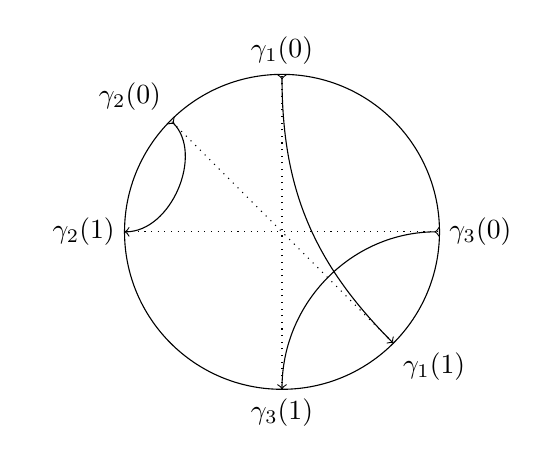
\begin{tikzpicture}
    % Circle
    \draw (0,0) circle (2cm);
    
    % Curve 1
    \draw[>->] (90:2cm) to[out=270, in=135] (-45:2cm);
    \node at (90:2cm) [above] {$\gamma_1(0)$};
    \node at (-45:2cm) [below right] {$\gamma_1(1)$};

    \draw[dotted] (-45:2cm) -- (135:2cm);
    
    % Curve 2
    \draw[>->] (135:2cm) to[out=-45, in=0] (180:2cm);
    \node at (135:2cm) [above left] {$\gamma_2(0)$};
    \node at (180:2cm) [left] {$\gamma_2(1)$};

    \draw[dotted] (180:2cm) -- (0:2cm);

    % Curve 3
    \draw[>->] (0:2cm) to[out=180, in=90] (-90:2cm);
    \node at (0:2cm) [right] {$\gamma_3(0)$};
    \node at (-90:2cm) [below] {$\gamma_3(1)$};

    \draw[dotted] (-90:2cm) -- (90:2cm);
\end{tikzpicture}
\begin{tikzpicture}
    % Circle
    \draw (0,0) circle (2cm);
    
    % Curve 1
    \draw[>->] (90:2cm) to[out=270, in=110] (0:2cm);
    \node at (90:2cm) [above] {$\gamma_1(0)$};
    % \node at (-45:2cm) [below right] {$\gamma_1(1)$};

    % \draw[dotted] (-45:2cm) -- (135:2cm);
    
    % Curve 2
    \draw[>->] (180:2cm) to[out=45, in=180] (150:1.5cm) to[out=0, in=0]  (180:2cm);
    % \node at (135:2cm) [above left] {$\gamma_2(0)$};
    \node at (180:2cm) [left] {$\gamma_2(0) = \gamma_2(1)$};

    \draw[dotted] (180:2cm) -- (0:2cm);

    % Curve 3
    \draw[>->] (0:2cm) to[out=180, in=90] (-90:2cm);
    \node at (0:2cm) [right] {$\gamma_1(1)=\gamma_3(0)$};
    \node at (-90:2cm) [below] {$\gamma_3(1)$};

    \draw[dotted] (-90:2cm) -- (90:2cm);
\end{tikzpicture}
\end{center}
If there is more than one segment, we can move $\gamma_1$ and $\gamma_2$ such that $\gamma_1(0)$ and $\gamma_2(1)$ remain fixed (so no other segments are affected) but $\gamma_2(0)$ is moved to $\gamma_2(1)$ (so necessarily $\gamma_1(1) \to - \gamma_2(1)$).
Then $\gamma_2$ can be contracted to the constant map $\gamma_1(1) = -\gamma_2(0) = -\gamma_2(1) = \gamma_3(0)$.
This means that we can eliminate $\gamma_2$ and fuse $\gamma_1$ and $\gamma_3$ into a single segment.
In particular, the index has decreased by two.
This argument has not quite proved that the parity of the index (even or odd) is a homotopy invariant, since there is still the possibility that some other tricky operation can decrease the index by an odd amount. 
But it should convince you none-the-less that the fundamental group of $\RP^3$, and hence $\SO(3)$, is $\bbZ_2$:
any loop with an even number of segments can be contracted to a point, whereas any loop with an odd number of segments can be reduced to a diameter.


\subsection{Definition}

\begin{definition}
\textup{\cite[3.1]{Warner1983}\cite[Definition~1.20]{Hall2015}} \\
A \emph{Lie Group} is a $G$ manifold with a group structure such that multiplication $\mu : (g,h) \mapsto gh$ and inversion $\iota : g \mapsto g^{-1}$ are smooth.
\end{definition}

Many familiar manifolds are also Lie groups in natural ways.
For example, the reals $\bbR$ under addition, the multiplicative group of the complex numbers $\bbC^\times$, and the circle $\bbS^1 = \{ z \in \bbC^\times \mid |z| = 1 \}$.
The product of two Lie groups is a Lie group, using the product manifold and product group structures.
This gives us euclidean space $\bbR^n$ with vector addition and the torus $\bbT^n = (\bbS^1)^n$ as further examples.

Left and right actions.
We can interchange left and right actions using inversion to make the opposite group.
Convention is to work primarily with left actions.
Hold off talking about general actions until quotients.

Many definition carry over naturally by requiring both a manifold-theory and a group-theory property.
For example
\begin{definition}
\textup{\cite[3.13]{Warner1983}} \\
A \emph{homomorphism of Lie groups} is a smooth map $\phi : G \to H$ that is also group homomorphism.
If it is also a diffeomorphism, then we say $\phi$ is an \emph{isomorphism of Lie groups}.
\end{definition}
On the other hand, sometimes a different concept is more appropriate for Lie theory.
In manifold theory one is mostly concerned with embedded submanifolds, while in Lie theory immersed submanifolds are more useful:
\begin{definition}
\textup{\cite[3.17]{Warner1983}, contrast~\cite[\S{}7.1]{Fulton2004}}\\
A \emph{Lie subgroup} $(H,\varphi)$ of a Lie group $G$ is a Lie group $H$ and injective immersion $\varphi : H \to G$ that is also a homomorphism.
It is called a \emph{closed Lie subgroup} if $\varphi(H)$ is further closed.
\end{definition}
An immersed manifold that is closed is an embedded submanifold. 

TODO: What is the proper order of material? 
In particular, the order of introducing Lie algebras and subgroups. 
Presumably you want to introduce examples early, which are mostly subgroups. 
Do you introduce subgroups before the examples?
Is it possible to introduce subgroups, quotients and covers without talking about the Lie algebra? Then introduce the Lie algebra and show how many of these it can grok.
That is certainly a differential geometry supremacist approach.


\subsection{Examples}

There are many interesting properties that Lie groups can possess, and we give a quick tour of them with examples.

All finite groups are also Lie groups using the discrete topology to make them $0$-dimensional manifolds.
These are not central examples of Lie groups, whose essential character is their `continuity', and they could reasonably be excluded by definition.
However we do not do so because they arise naturally.
For example, we have seen that the $\SO(3)$ is the component of $\O(3)$ that contains the identity.
In fact $\O(3)$ is the product of $\SO(3)$ and $C_2$ the group with two elements.
Generalising, the identity component $G_0$ of a Lie group $G$ is a Lie group.
To prove this, note that $II = I$ and $I^{-1} = I$, so the images of $G_0\times G_0$ under multiplication and $G_0$ under inversion are both contained in $G_0$.
If $g$ belongs to another connected component $G_1$ then multiplication with $g$ is a diffeomorphism between $G_0$ and $G_1$.
In this way, every Lie group with finitely many connected components is the product of its identity component and a finite group.
For this reason we usually consider connected Lie groups of positive dimension.

Perhaps the most important category of Lie group are the matrix Lie groups~\cite[Definition~1.4]{Hall2015}.
First we have the general linear group $\GL(n,\bbC)$, the set of $n\times n$ invertible matrices with complex entries.
This can be considered as an open subset of $\bbC^{n^2}$, so it is a manifold. And just as for $\O(3)$ the group operation is polynomial and group inversion is rational without zeroes of the denominator, hence both are smooth.
A matrix group is any closed Lie subgroup of $\GL(n,\bbC)$.
As a special case we have the real matrix groups, which are subsets of the (real) matrix group $\GL(n,\bbR)$.

We have already seen the real matrix groups $\O(3)$ and $\SO(3)$.
As the notation suggests, these belong to families indexed by the size of the matrices.
We have the following families of matrix groups
\begin{align*}
\SL(n,\bbC) &= \{ A \in \GL(n,\bbC) \mid \det A = 1 \} \\
\SL(n,\bbR) &= \{ A \in \GL(n,\bbR) \mid \det A = 1 \} \\
\U(n) &= \{ A \in \GL(n,\bbC) \mid \bar{A}^T A = I \} \\
\SU(n) &= \{ A \in \U(n) \mid \det A = 1 \} \\
\O(n) &= \{ A \in \GL(n,\bbR) \mid A^T A = I \} \\
\SO(n) &= \{ A \in \O(n) \mid \det A = 1 \}.
\end{align*}
If we give $\bbC^n$ the standard inner product $\langle v,w \rangle = \bar{v}^Tw$ then unitary matrices are exactly the linear transformations that preserve it.
In this way the orthogonal groups are the real counterparts to the unitary groups.
The following trick shows that $\U(n)$ is compact: As a vector in $\bbC^{n^2}$ the square of the norm of $A \in \U(n)$ is $\tr(\bar{A}^T A) = \tr I = n$, thus $\U(n)$ is bounded.
Thus all closed subsets, such as $\SU(n), \O(n),\SO(n)$, are also compact.

There are also the symplectic groups.
Like $\U$ and $\O$ they preserve a bilinear form.
Let 
\[
\Omega = \begin{pmatrix}
0 & I_n \\ - I_n & 0
\end{pmatrix}
\]
be a $2n\times 2n$ matrix in block form and define
\begin{align*}
\Sp(2n,\bbC) &= \{ A \in \GL(2n,\bbC) \mid A^T\Omega A = \Omega \} \\
\Sp(2n,\bbR) &= \{ A \in \GL(2n,\bbR) \mid A^T\Omega A = \Omega \} \\
\Sp(n) &= \Sp(2n,\bbC) \cap \U(2n).
\end{align*}
The notation around $\Sp(n)$ is a bit confusing, but the point is to make a compact group.
Indeed $\Sp(n)$ is called the compact symplectic group.

Together, these examples are called the classical groups and they will figure prominently in the classification of Lie groups.
There are of course many other matrix Lie groups.
One could consider groups of matrices preserving other bilinear forms. 
For a concrete example, the subset of diagonal matrices of any of the classical groups is again a matrix group.
In $\U(n)$ the diagonal subgroup is $\{\operatorname{diag}(\lambda_1,\dots,\lambda_n)\}$ with $|\lambda_i| = 1$.
We see that this is isomorphic to $\bbT^n$.
The standard terminology is that a Lie group that is isomorphic to a matrix group is called a linear group.
In other words, $\bbT^n$ which is defined as the product of circles, is a linear group but not a matrix group.
Similarly $\bbR$ is a linear group because we can consider real matrices of the form
\[
\begin{pmatrix}
1 & a \\
0 & 1
\end{pmatrix}.
\]
The result of multiplying two such matrices is the add the off-diagonal term.

TODO: Complex Lie groups. $\SL(n,\bbC)$ is a complex Lie group but $\U(n)$ is not.
A similar direction that we will not explore is linear algebraic groups.
These are matrix groups whose defining equations are polynomial.
This means that they can be defined over any field, not just $\bbC$ and $\bbR$.


As in group theory, we have abelian and non-abelian groups.
Abelian Lie groups include $\bbR^n$ and $\bbT^n$ and $\O(3)$ and $\SO(3)$ are examples of non-abelian groups.
% Similarly, consider the Heisenberg group
% \[
% H = \begin{pmatrix}
% 1 & a & b \\
% 0 & 1 & c \\
% 0 & 0 & 1
% \end{pmatrix}
% \]
% for $a,b,c\in \bbR$.


\subsection{Subgroups}


\subsection{Quotients}


\subsection{Covers}


\subsection{Mauer-Cartan forms}
Should we have such a section? Sharpe and Ivey has it, but I don't think Warner puts as much emphasis on it.


\subsection{Simple Lie groups}
We should give a refined version of the classification problem: to find simply-connected simple Lie groups.



\section{Lie algebra}

TODO: maybe the angle here should be that Lie groups are homogeneous manifolds, so it makes sense to focus on neighbourhoods of the identity.
Maybe the result that a neighbourhood of the identity generates a connected Lie group \cite[3.18]{Warner1983}.
Then talk about the exponential map which is a local diffeomorphism from $\frg$ to $G$ at $e$.
This frames the section: we have the internal generation of a Lie group, how do we externally generate it from the tangent space?

\subsection{Lie Bracket}
Lie bracket coming from the adjoint action.
There are lots of names for conjugation, eg the power notation, Sharpe uses $\mathbf{Ad}$, Warner $a$. I think a two letter operator, eg $\operatorname{Cn(g)}$ would be best. Wikipedia uses $\Psi$. There's also the question of $\ad(x)$ or $\ad_x$.
I think this one shows most clearly how the bracket is encodes some infinitesimal information of the group operation.

This is Lie bracket of left-invariant vector fields.


\subsection{Examples}
Matrix vs abstract Lie algebras
Bracket of matrix Lie algebras is commutator

Lie algebras of all the classical groups.


\subsection{Correspondences}

Stuff like Lie group homomorphisms inducing Lie algebra homomorphisms.
ideals and subalgebras

I found this pdf \url{https://www.cis.upenn.edu/~cis6100/cis610-15-sl17.pdf} that connects metrics on the Lie group with inner products on the Lie algebra.


\subsection{Ado's theorem}
\url{https://terrytao.wordpress.com/2011/05/10/ados-theorem/}
This seems elementary, and introduces all the important classes of Lie algebras: sovlable, nilpotent, etc. But it defines complex Lie algebras at the outset? Maybe we already need to consider real vs complex Lie algebras, complexifications, etc.

Maybe we only need a weaker version, that all simple Lie algebras are matrix?
Indeed, the adjoint representation works for centerless Lie algebras.



\section{Classification of Lie algebras}

TODO: make sections.

I would like to gather up at the start all the structure that we need. I am thinking here in particular of inner products and Weyl reflections.

The introduction of \url{https://terrytao.wordpress.com/2013/04/27/notes-on-the-classification-of-complex-lie-algebras/} is nice.

From \url{https://en.wikipedia.org/wiki/Killing_form} there seems to be a close connection between the Killing form and decompositions of Lie algebras:
\begin{itemize}
\item On a simple Lie algebra any invariant symmetric bilinear form is a scalar multiple of the Killing form.
\item The Killing form is also invariant under automorphisms of the Lie algebra
\item The Cartan criterion states that a Lie algebra is semisimple if and only if the Killing form is non-degenerate.
\item The Killing form of a nilpotent Lie algebra is identically zero.
\item Ideals that intersect only trivially are orthogonal.
\end{itemize}
This paper \url{https://math.uchicago.edu/~may/REU2012/REUPapers/Bosshardt.pdf} from Uchicago undergrad summer projects 2012 seems to go hard on the Killing form.

If we are focused on simple Lie algebras, then can we avoid the other types?

I don't want to build representation theory.
I think we only really need the adjoint representation and $\sl(2,\bbC)$-representations.
Maybe we can understand them as a special type of subspace.


\subsection{Cartan subalgebra}
A point of difficulty seems to be Cartan subalgebras.
In fact there are several, somewhat incompatible definitions in the literature (in different cases) to suit different circumstances.
Hall takes the simplest definition: a maximal commuting subalgebra of diagonalizable elements.
This immediately gives you a root space decomposition, commuting implies simultaneously diagonalizable.
The existence is rather easy too, but only because he begins with a real compact form for the complex semisimple algebra.
FH takes the same definition, but in Appendix D proves existence through regular elements.

Knapp takes a more principled approach, asking what we should require of a subalgebra to get a decomposition like we see in the standard examples, p83.
It takes the more general starting point of a nilpotent subalgebra h.
Not all of them lead to a really nice decomposition, but somehow maximal ones do, and these we call Cartan subalgebras.
The drawback is that we don't have diagonalizability at the start, so we have to work with generalised eigenspaces, see Prop 2.5 p88.
Here too the existence relies on regular elements Theorem 2.9.

Knapp Chapter 4 comes back to Hall's point: Cor 4.26 a compact Lie group has negative definite Killing form. Prop 4.27, gives an argument for the converse!

What drew me to Knapp though was the discussion of real simple Lie algebras.
In particular, how complex Lie algebras can arise from real ones.
The two extremes are the split real form and the compact real form.
These are constructed explicitly Cor 6.10 and Thm 6.11, but they require the root decomposition.
Other real forms (and these ones too) are described by a Cartan involution. 
It is a vector space sum on which the Killing form is resp pos and neg definite (6.26) and the brackets are behaved (6.24).
Perhaps this could be the basis of a direct proof of a compact real form.
After some googling, this was suggested by Cartan 1929 to simplify the proof, and there's a paper by Richardson (?) that carries it out.
But it's not as simple as it sounds.

Another thing to consider would be to only classify compact lie groups.
This has the advantage that then the compact real form is a natural part of the set-up.
You get basically the same list at the end.
It has most of the features you want to consider.
And then maybe you can carry the classification all the way back to the level of real Lie groups, without so much of the messy involution stuff at the end.
Go deeper on compact Lie groups; apparently their universal covers are compact, you can understand the quotient theory well.
It does fell like a limitation, when we are so close to getting all complex semisimple Lie algebras.

\bibliographystyle{alpha} 
\bibliography{LieGroups}

\end{document}

